% !TEX TS-program = pdflatex
% !TEX encoding = UTF-8 Unicode

% This is a simple template for a LaTeX document using the "article" class.
% See "book", "report", "letter" for other types of document.

\documentclass[11pt]{article} % use larger type; default would be 10pt

\usepackage[utf8]{inputenc} % set input encoding (not needed with XeLaTeX)

%%% Examples of Article customizations
% These packages are optional, depending whether you want the features they provide.
% See the LaTeX Companion or other references for full information.

%%% PAGE DIMENSIONS
\usepackage{geometry} % to change the page dimensions
\geometry{a4paper} % or letterpaper (US) or a5paper or....
% \geometry{margin=2in} % for example, change the margins to 2 inches all round
% \geometry{landscape} % set up the page for landscape
%   read geometry.pdf for detailed page layout information

\usepackage{graphicx} % support the \includegraphics command and options

% \usepackage[parfill]{parskip} % Activate to begin paragraphs with an empty line rather than an indent

%%% PACKAGES
\usepackage{booktabs} % for much better looking tables
\usepackage{array} % for better arrays (eg matrices) in maths
\usepackage{paralist} % very flexible & customisable lists (eg. enumerate/itemize, etc.)
\usepackage{verbatim} % adds environment for commenting out blocks of text & for better verbatim
\usepackage{subfig} % make it possible to include more than one captioned figure/table in a single float
\usepackage{graphicx}
\usepackage{float}
\usepackage[]{algorithm2e}
% These packages are all incorporated in the memoir class to one degree or another...

%%% HEADERS & FOOTERS
\usepackage{fancyhdr} % This should be set AFTER setting up the page geometry
\pagestyle{fancy} % options: empty , plain , fancy
\renewcommand{\headrulewidth}{0pt} % customise the layout...
\lhead{}\chead{}\rhead{}
\lfoot{}\cfoot{\thepage}\rfoot{}

%%% SECTION TITLE APPEARANCE
\usepackage{sectsty}
\allsectionsfont{\sffamily\mdseries\upshape} % (See the fntguide.pdf for font help)
% (This matches ConTeXt defaults)

%%% ToC (table of contents) APPEARANCE
\usepackage[nottoc,notlof,notlot]{tocbibind} % Put the bibliography in the ToC
\usepackage[titles,subfigure]{tocloft} % Alter the style of the Table of Contents
\renewcommand{\cftsecfont}{\rmfamily\mdseries\upshape}
\renewcommand{\cftsecpagefont}{\rmfamily\mdseries\upshape} % No bold!

%%% END Article customizations

%%% The "real" document content comes below...

\title{Adaptive Quadrature Methods}
\author{Nicholas Padinha}
%\date{November 2014} % Activate to display a given date or no date (if empty),
         % otherwise the current date is printed 

\begin{document}

\maketitle
\begin{abstract}
\textit{Adaptive quadrature} refers to a family of techniques bringing the divide-and-conquer and Richardson extrapolation strategies to bear on the problem on numerical integration. Any integration scheme can hypothetically be given an adaptive version if there is a suitable error estimator available for that scheme. Here we focus on the adaptive version of Simpson's rule. The rule requires no precomputation in selecting subintervals to integrate over and demonstrably outperforms Simpson's rule in accuracy on bad integrals.
\end{abstract}
\listoffigures

\section{Introduction}

\textit{Adaptive quadrature} is a general method for improving the accuracy of a quadrature rule (i.e., numerical integration scheme). A sketch of the idea is as follows: We select a quadrature rule with an a priori error estimator. We apply the quadrature to the function we want to integrate and estimate the error. If the error meets a certain condition (for example, exceeding a certain tolerance), we subdivide the interval and repeat the process on each subinterval. We hope to subdivide those regions more which make greater contributions to the total error, while settling for larger intervals when the local error is small.

An adaptive Simpson's method was proposed in 1962 and by now the idea has been applied to a wide range of quadrature rules. The subdivision criterion which appears in the adaptive Simpson's method is to subdivide when the discrepancy between a single approximation (on [a,b]) and the sum of two approximations (on [a,c] and [c,b]) exceeds a certain tolerance. The discrepancy tolerance is derived by setting a tolerance for the total error and then applying Simpson's rule's error estimate in the single-interval and composite-interval cases (see Section 3 for details).

In this report we will present the algorithm for adaptive Simpsons quadrature and compare it procedurally with composite Simpson quadrature in order to highlight the difference. The explanation and error analysis of the quadrature appear next, followed by empircal observations. These consist of tables of integration results obtained from composite Simpson quadrature and adaptive Simpson quadrature, tables comparing number of intervals and computations for each method for the same problems, and plots demonstrating this information against the graphs of the functions being integrated.

\section{Adaptive Simpson Quadrature---Explanation and Analysis}
(This analysis follows the explanation given in [3].) Let $f$ be a given integrable function. Define
$$S(a,b) = \frac{b-a}{6}\left(f(a) +4f\left(\frac{a+b}{2}\right) + f(b)\right)$$
and
$$E(a,b) = -\frac{1}{90}\left(\frac{b-a}{2}\right)^5 f^{(4)}(a) + \dots.$$
Then recall that Simpson's method evaluates the integral of $f$ on $[a,b]$ as
$$I_= \int_a^b f dx = S(a,b) +E(a,b).$$
Let $S_1 = S(a,b)$, let $E_1 = E(a,b)$, and let $h = b-a$. Then also let $c = (b+a)/2$. Applying Simpson's method to both of
$[a,c]$ and $[c,b]$ we obtain
$$I  = S(a,c) + S(c,b) + E(a,c) + E(c,b).$$
Write $S_2 = S(a,c) + S(c,b)$ and $E_2 = E(a,c) + E(c,b)$. Then under the simplifying assumption that $f^(4) = C$, a constant, on
$[a,b]$, we have
$$E_2 = \frac{1}{16}\left(-\frac{1}{90} \left(\frac{h}{2}\right)^5 C\right) = \frac{1}{16}E_1.$$
Now subtracting one value obtained for $I$ from the other, we arrive at the equation
$$S_2 - S_1 = E_1 - E_2 = 15E_2$$
which gives us
$$I = S_2 + \frac{1}{15}(S_2 - S_1).$$
Hence, if $\epsilon$ is our error tolerance for $I$, then we see that requiring
$$\frac{1}{15}\left|S_2 - S_1\right| < \epsilon$$
will guarantee that $I$ is correct to within $\epsilon$.\\
Therefore, we will take $ S_2 + \frac{1}{15}(S_2 - S_1)$ as the value of the integral on $[a,b]$ if the above criterion is met,
and otherwise we will split the interval $[a,b]$ into intervals $[a,c]$ and $[c,b]$, applying the same procedure to each subinterval. In 
order to keep our total error within $\epsilon$, we clearly must require that the errors on $[a,c]$ and $[c,b]$ are within $\epsilon/2$.
The procedure should remind the reader of Romberg integration, in the sense that $S_2 + \frac{1}{15}(S_2 - S_1)$ is the reuslt
obtained by applying the extrapolation process to Simpson's rule once.\\
In practice, we will handle this with a recursive function. The algorithm is presented in pseudocode in the next section.

\section{Adaptive Simpson Quadrature---Algorithm}
For the description of the adaptive Simpson quadrature algorithm, we take for granted Simpson's rule for a single interval.\\


\begin{algorithm}[H]
 \KwData{a function $F$, an interval $[A,B]$ on which to integrate, a tolerance $\epsilon$}
 \KwResult{an approximation for the integral of $f$ on $[a,b]$}
 Set $W$ equal to Simpsons(F,A,B)\;
Set $C$ equal to (A+B)/2\;
Set $L$ equal to Simpsons(F,A,C)\;
Set $R$ equal to Simpsons(F,C,B)\;

 \eIf{$|L + R - W| \leq 15\epsilon$ }{
   Return $L + R + (L+R-W)/15$\;  
 }{Return AdaptiveSimpsons($F,A,C,\epsilon/2$) + AdaptiveSimpsons($F,C,B,\epsilon/2$)\;}
 \caption{Adaptive Simpson Quadrature}
\end{algorithm}

(See [2] for more details.)
\section{Data---Figures}
\begin{center}
\begin{figure}[H]
  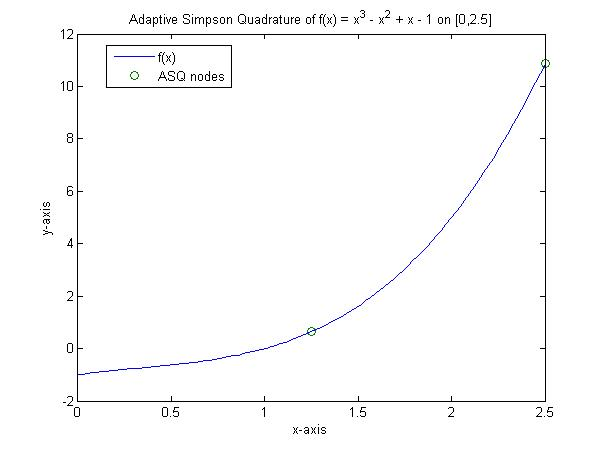
\includegraphics[width=450px]{graphics/cubic_integral_adaptive_simps.jpg}
  \caption[ASQ applied to a cubic function]{ASQ applied to a cubic function. Simpson's rule obtains an exact value for this integral, so the adaptive rule does not 
  have to subdivide the interval at all.}
\end{figure}

\begin{figure}[H]
  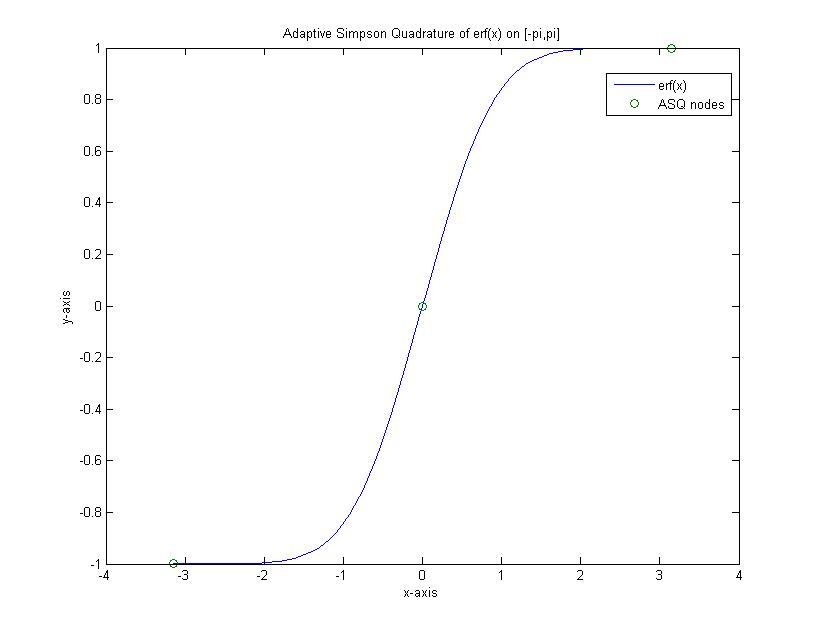
\includegraphics[width=550px]{graphics/erf_adaptive_simps1.jpg}
  \caption[ASQ applied to the error function on a symmetric interval]{ASQ applied to the error function on a symmetric interval. As a consequence of the symmetry of this function about zero,
  the adaptive scheme finds the value of the integral--zero--without subdivision.}
\end{figure}

\begin{figure}[H]
\centering
  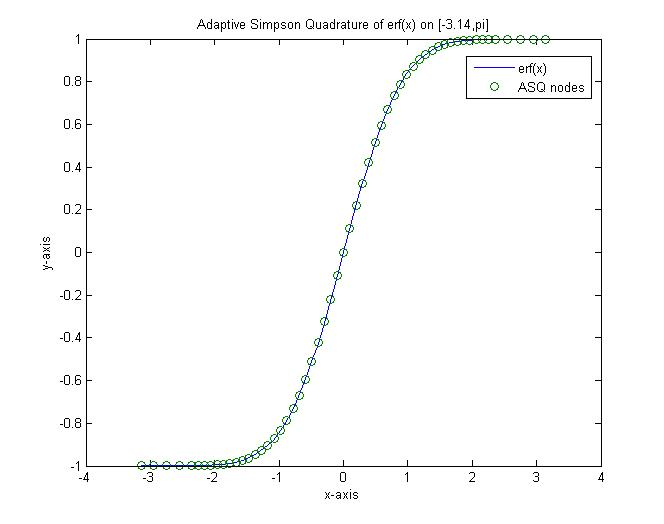
\includegraphics[width=550px]{graphics/erf_adaptive_simps2.jpg}
  \caption[ASQ applied to the error function on an asymmetric interval]{ASQ applied to the error function on an asymmetric interval. By shifting the values of the endpoints slightly we break the symmetry, and now ASQ needs many subdivisions to find a satisfactory approximation. Perhaps surprisingly, slightly more intervals are needed where the values of the function change the least. See the next section for the results of CSQ on this function.}
\end{figure}

\begin{figure}[H]
\centering
  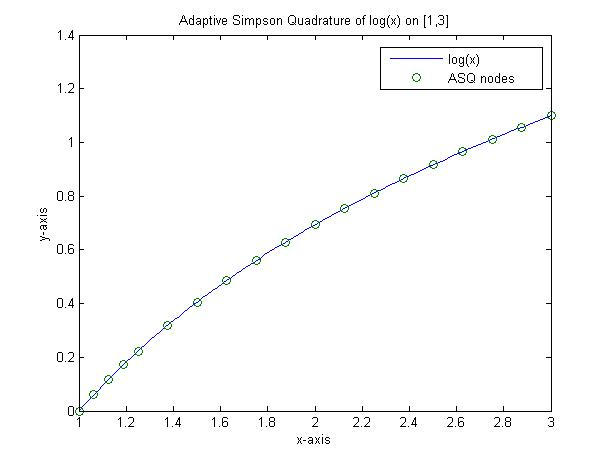
\includegraphics[width=450px]{graphics/log_adaptive_simps.jpg}
  \caption[ASQ applied to the natural logarithm]{ASQ applied to the natural logarithm. For particularly well-behaved integrals, the intervals found by ASQ end up being evenly-spaced or close to it.}
\end{figure}

\begin{figure}[H]
  \centering
  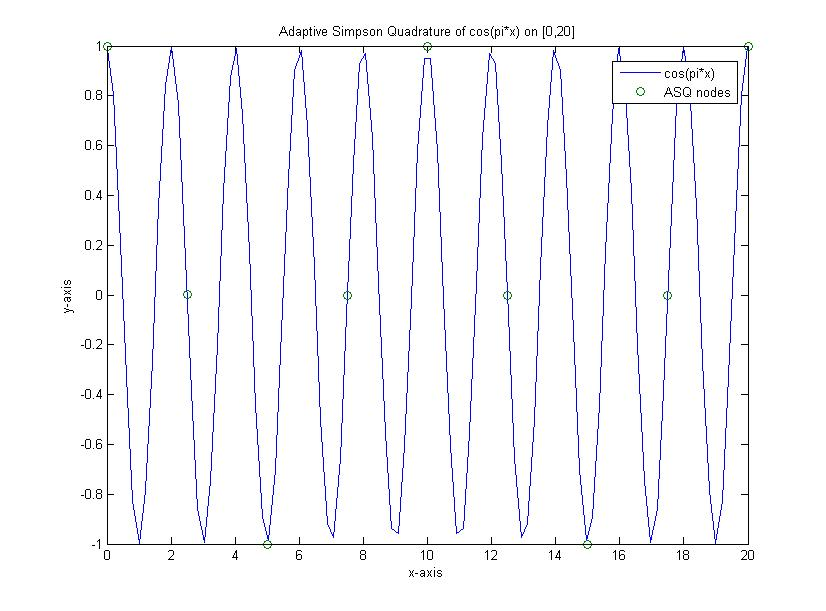
\includegraphics[width=500px]{graphics/cospix_adaptive_simps.jpg}
  \caption[ASQ applied to $\cos(\pi x)$]{ASQ applied to $\cos(\pi x)$. Ultimately, ASQ finds evenly-spaced intervals. However, one easily sees why evenly-spaced intervals chosen \textit{a priori} could become a problem when numerically integrating a periodic function. Compare this figure to the next.}
\end{figure}

\begin{figure}[H]
  \centering
  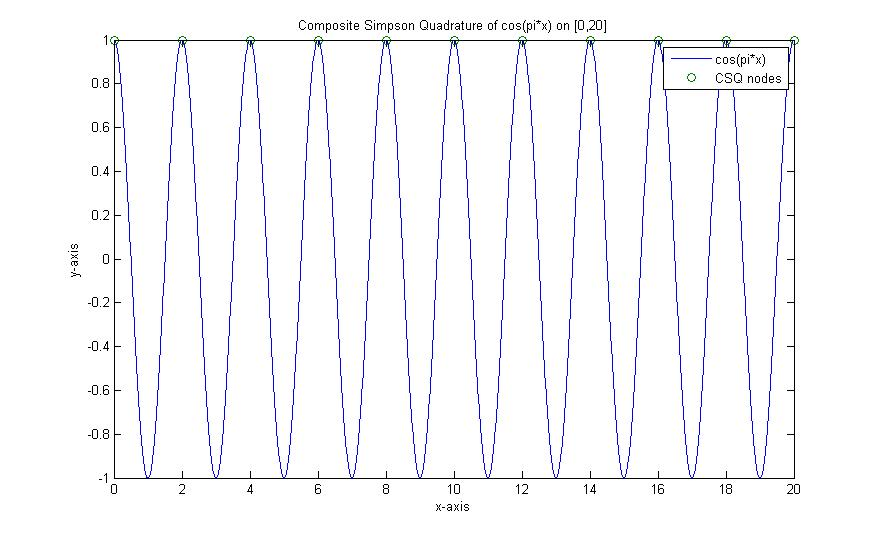
\includegraphics[width=500px]{graphics/cospix_composite_simps.jpg}
  \caption[CSQ applied to $\cos(\pi x)$]{CSQ applied to $\cos(\pi x)$. By carelessly selecting evenly-spaced intervals for composite Simpson quadrature, we accidentally chose the crest of every wave as the sampling point! Refer to Tables 1 and 2 for numerical data on this integral.}
\end{figure}
\end{center}

\section{Data---Tables}

\begin{table}[H]
    \centering
    \begin{tabular}{lccr}
    \hline
    
        \textbf{ f }
        
           &
        
    
        \textbf{ I }
        
           &
        
    
        \textbf{ Simpson }
        
           &
        
    
        \textbf{ Adaptive Simpson }
        
     
    \\
    \hline
    
        
            cubic
             
               &
            
        
            [0:2.5]
             
               &
            
        
            2.6855662247
             
               &
            
        
            5.1822916667
            
        
        \\
    
        
            erf
             
               &
            
        
            [$-\pi$:$\pi$]
             
               &
            
        
            -0.6961222732
             
               &
            
        
            0.0000000000
            
        
        \\
    
        
            erf
             
               &
            
        
            [-3.14:$\pi$]
             
               &
            
        
            -0.6943581282
             
               &
            
        
            0.0015926394
            
        
        \\
    
        
            log
             
               &
            
        
            [1:3]
             
               &
            
        
            1.0601181852
             
               &
            
        
            1.2958368650
            
        
        \\
    
        
            cos(pi*x)
             
               &
            
        
            [1:3]
             
               &
            
        
            -2.0489218097
             
               &
            
        
            0
            
        
        \\
    
    \hline
    \end{tabular}
    \caption{Integrals computed by composite Simpson's rule (20 intervals) are compared with those computed by adaptive Simpson's 	
    rule.}
    \label{tab:ASQvsCSQ}
\end{table}

\begin{table}[H]
    \centering
    \begin{tabular}{lr}
    \hline
    
        \textbf{ N }
        
           &
        
    
        \textbf{ CSQ(N) }
        
     
    \\
    \hline
    
        
            2
             
               &
            
        
            0.00000000000
            
        
        \\
    
        
            3
             
               &
            
        
            20.00000000000
            
        
        \\
    
        
            4
             
               &
            
        
            -3.33333333333
            
        
        \\
    
        
            5
             
               &
            
        
            -6.66666666667
            
        
        \\
    
        
            6
             
               &
            
        
            16.00000000000
            
        
        \\
    
        
            7
             
               &
            
        
            -0.00000000000
            
        
        \\
    
        
            8
             
               &
            
        
            -1.04669631628
            
        
        \\
    
        
            9
             
               &
            
        
            -0.00000000000
            
        
        \\
    
        
            10
             
               &
            
        
            -2.04892180972
            
        
        \\
    
        
            11
             
               &
            
        
            20.00000000000
            
        
        \\
    
        
            12
             
               &
            
        
            -1.72197183808
            
        
        \\
    
        
            13
             
               &
            
        
            -0.00000000000
            
        
        \\
    
        
            14
             
               &
            
        
            -1.08745470782
            
        
        \\
    
        
            15
             
               &
            
        
            -0.00000000000
            
        
        \\
    
        
            16
             
               &
            
        
            -0.66666666667
            
        
        \\
    
        
            17
             
               &
            
        
            0.00000000000
            
        
        \\
    
        
            18
             
               &
            
        
            -0.45089524089
            
        
        \\
    
        
            19
             
               &
            
        
            -0.00000000000
            
        
        \\
    
        
            20
             
               &
            
        
            -0.35566270056
            
        
        \\
    
        
            21
             
               &
            
        
            -6.66666666667
            
        
        \\
    
        
            22
             
               &
            
        
            -0.32100608691
            
        
        \\
    
        
            23
             
               &
            
        
            0.00000000000
            
        
        \\
    
        
            24
             
               &
            
        
            -0.31385179667
            
        
        \\
    
        
            25
             
               &
            
        
            -0.00000000000
            
        
        \\
    
    \hline
    \end{tabular}
    \caption{Results from composite Simpson quadrature applied to $\cos(\pi x)$ on $[0,20]$. The number of intervals, $N$, ranges from 2 to 25, demonstrating the high errors that can result from applying CSQ to a periodic function.}
    \label{tab:cospix}
\end{table}
\section{Explanation of Data and Conclusions}
The cubic function demonstrates clearly that the adaptive method agrees with the composite method for a polynomial of sufficiently small degree—of course, the value found by Simpson’s rule is actually the exact value of the integral. The error function reveals some of the behavior of the adaptive versus the naïve scheme. On the symmetric interval, the integral is 0 and adaptive Simpson’s finds the same exact value as composite Simpson’s without extra subdivisions. On the asymmetric interval, adaptive Simpson’s needs extra subdivisions to compute the integral correctly, and the value found is not exactly zero but in fact closer to the minimum floating point allowed by the running architecture.\\
Figures 5 and 6 and Table 2 further demonstrate the usefulness of adaptive quadrature. Given a periodic function, such as $f(x) = \cos(\pi x)$, manually choosing subdivision nodes for composite Simpson's rule requires careful attention to the location of the waveform's crests and troughs so as not to wildly over- or underestimate the integral, and attempting to find the integral as the limit of composite Simpson's rule as the number of intervals goes up can be a very slowly-converging process. For a function represented as a Fourier or generalized Fourier sequence, this can mean that a very large number of intervals are required to make composite Simpson's rule acceptable. 



\section{References}
\begin{enumerate}
\item Calvetti, D.; Golub, G. H.; Gragg, W. B. and Reichel, L. "Computation of Gauss-Kronrod Quadrature Rules." Math. Comput. 69, 1035-1052, 2000. 

\item http://www.mathworks.com/moler/quad.pdf

\item Cheney, W.; Kincaid, D. Numerical Mathematics and Computing, 7th Edition.
\end{enumerate}

\end{document}
